\chapter{Event Reconstruction}
\label{chap:reco}

This chapter describes the reconstruction of events collected by the CMS
detector. The $\PH \to \Pgt\Pgt$ analysis uses almost every object measured in
CMS and makes use of information from every sub-detector. 
Section \ref{sec:vertex} describes the reconstruction of the
primary vertex using measured tracks in the event. Sections \ref{sec:electrons}
and \ref{sec:muons} describe the reconstruction of the electrons and muons in
the event combining the tracks with information from the \ac{ECAL} and muon
chambers respectively. Section \ref{sec:jets} describes the reconstruction and
treatment of jets, followed by section \ref{sec:met} describing how the missing
energy of the event is then calculated. Finally the reconstruction of hadronic taus
is described in section \ref{sec:taus}.

In addition to the reconstruction of the objects used in the $\PH \to \Pgt\Pgt$
analysis, the final section of this chapter contains a description of a tool of
great importance to this analysis - a likelihood based reconstruction of the
di-tau pair mass, described in section \ref{sec:svfit}.

\section{Primary Vertex Reconstruction}
\label{sec:vertex}

The reconstruction of the \ac{PV} of the event allows us to identify the hard
$pp$ interaction over the other vertices from multiple $pp$ collisions in the same
bunch crossing, known as \ac{PU}. In 2011 data at CMS there was an average of 9
\ac{PU} vertices and in 2012 data the average was even higher at 21. Correct
identification of the \ac{PV} also allows us to distinguish "prompt" production of
particles, i.e. production at the \ac{PV} from the hard interaction, from
in-flight decays of hadrons or photon conversions.  

The vertices are reconstructed using the tracks in the inner
tracker. A clustering algorithm, called the \ac{DA} algorithm
\cite{DetAnnealing}, is used to assign tracks to their most likely 
vertex. Each vertex is seeded by at least 2 tracks separated in z by less than
$1 \cm$ at the point of closest approach to the z axis.
The most likely position of each vertex is then determined using the
adaptive vertex fitter \cite{adaptivevertex}. In
this fitter each track is assigned a weight, $w_{i}$, which is close to 1 for tracks which
are highly compatible with the fitted vertex position and close to 0 for tracks with low
compatibility. These weights are used to define the number of degrees of freedom
for the fit as: $n_{dof}^{vertex} = 2\sum_{i}^{\text{tracks}}w_{i}-3$. This
variable is an assessment of the mutual compatibility of the component tracks of
the vertex, and is used to distinguish real $pp$ interactions from
mis-reconstructed vertices. For most analyses, quality cuts \cite{CMS-PAS-TRK-10-005} on each vertex are
applied as follows:
\begin{itemize}
\item The distance in the z direction from the vertex to the nominal interaction
point must be smaller than $24\cm$. 
\item The corresponding distance in the transverse plane must be smaller than
$2\cm$.
\item $n_{dof}^{vertex} > 4$.
\end{itemize}

The \ac{PV} is taken to be the vertex with the highest sum squared $\pt$ of its
associated tracks. 

\section{Electrons}
\label{sec:electrons}

Electrons are reconstructed by matching \ac{ECAL} deposits with tracks from the
inner tracker. This is made more difficult by the fact that the electrons
undergo bremsstrahlung when interacting with the material of the tracker
detectors. The photons produced can also convert to $\Pep\Pem$ pairs before
reaching the \ac{ECAL}. This means that the energy deposited in the \ac{ECAL} 
can be spread out in the $\phi$ direction. Hence dedicated algorithms are used
to combine the energy deposits from both the initial electron and the
bremsstrahlung products, known as ``supercluster'' algorithms \cite{ElectronReco}.

The algorithms used are different for electrons in the barrel and endcaps, in
order to be optimal for the different geometries. In both cases, a clustering is performed
in the $\eta-\phi$ plane starting from the \ac{ECAL} crystal with the most energetic deposit, and
continuing outwards to the surrounding crystals until there are no more
unclustered crystals above a certain energy threshold. In the barrel, the
``hybrid'' clustering algorithm is used. In this algorithm the seed crystal has
$\Et > 1 \GeV$ and the clustering is performed in a ``domino'' of $3\times1$ or
$5\times1$ crystals, with additional dominoes (which attempt to collect
radiation deposits) stepping in both $\phi$
directions around the seed up to $\Delta\phi\approx0.3$. The threshold upon
which the clustering ends is $100\MeV$. In the endcaps the clustering algorithm
is the ``Multi5$\times$5'' algorithm using $5\times5$ arrays of crystals within
$\Delta\eta<0.07$ and $\Delta\phi<0.3$.

The energy-weighted average position of the supercluster is computed, and this
position is the equivalent of the impact point in the \ac{ECAL} of a
non-radiating electron with energy equal to the supercluster energy. This is
matched to a compatible hit in a loose $\phi$-$z$ search region 
in the in the first pixel layer, under the
hypothesis that the electron could be either charge. If a compatible hit is
found, the hit in the first layer is used to update the estimated electron
trajectory which would result in hits in the outer layers. This seeds the
reconstruction of the electron trajectory through the Silicon Strip Tracker
using the \ac{GSF} algorithm \cite{GSFalgorithm}. This provides an additional momentum measurement
which is used to improve the electron energy resolution. 

%Backgrounds to electrons are expected to originate
%in hadronic jets, for example where a $\Pgpz$ and $\Pgppm$ overlap, or where a
%$\Pgppm$ showers early in the \ac{ECAL}.
% read the paper and understand better what these backgrounds are!! pions?
Electron ID criteria are used in many analyses to improve the efficiency of
selecting real electrons over backgroundsi (which tend to originate from
hadronic jets). The most commonly used variables are \cite{Baffioni:2006cd}:

\begin{itemize}
\item $\Delta\eta_{\text in}$ and $\Delta\phi_{\text in}$, the separation in the
$\eta$ and $\phi$ between the supercluster and track direction
evaluated at the \ac{PV} position and extrapolated to the \ac{ECAL} (generally
smaller for prompt electrons).
\item $\sigma_{i\eta i\eta}$, the energy-weighted $\eta$ width of the cluster.
This is typically small for prompt electrons, which have a more localised
cluster.
\item $H/E$, the ratio of hadronic to electromagnetic energy in the region of
the seed cluster (generally lower for prompt electrons).
\end{itemize}

Figure \ref{fig:electronID} shows the distributions of these variables in both simulated
electrons and jets in the barrel, and it can clearly be seen that these variables provide
excellent discrimination power:

\begin{figure}
\begin{center}
\subfloat[]{
    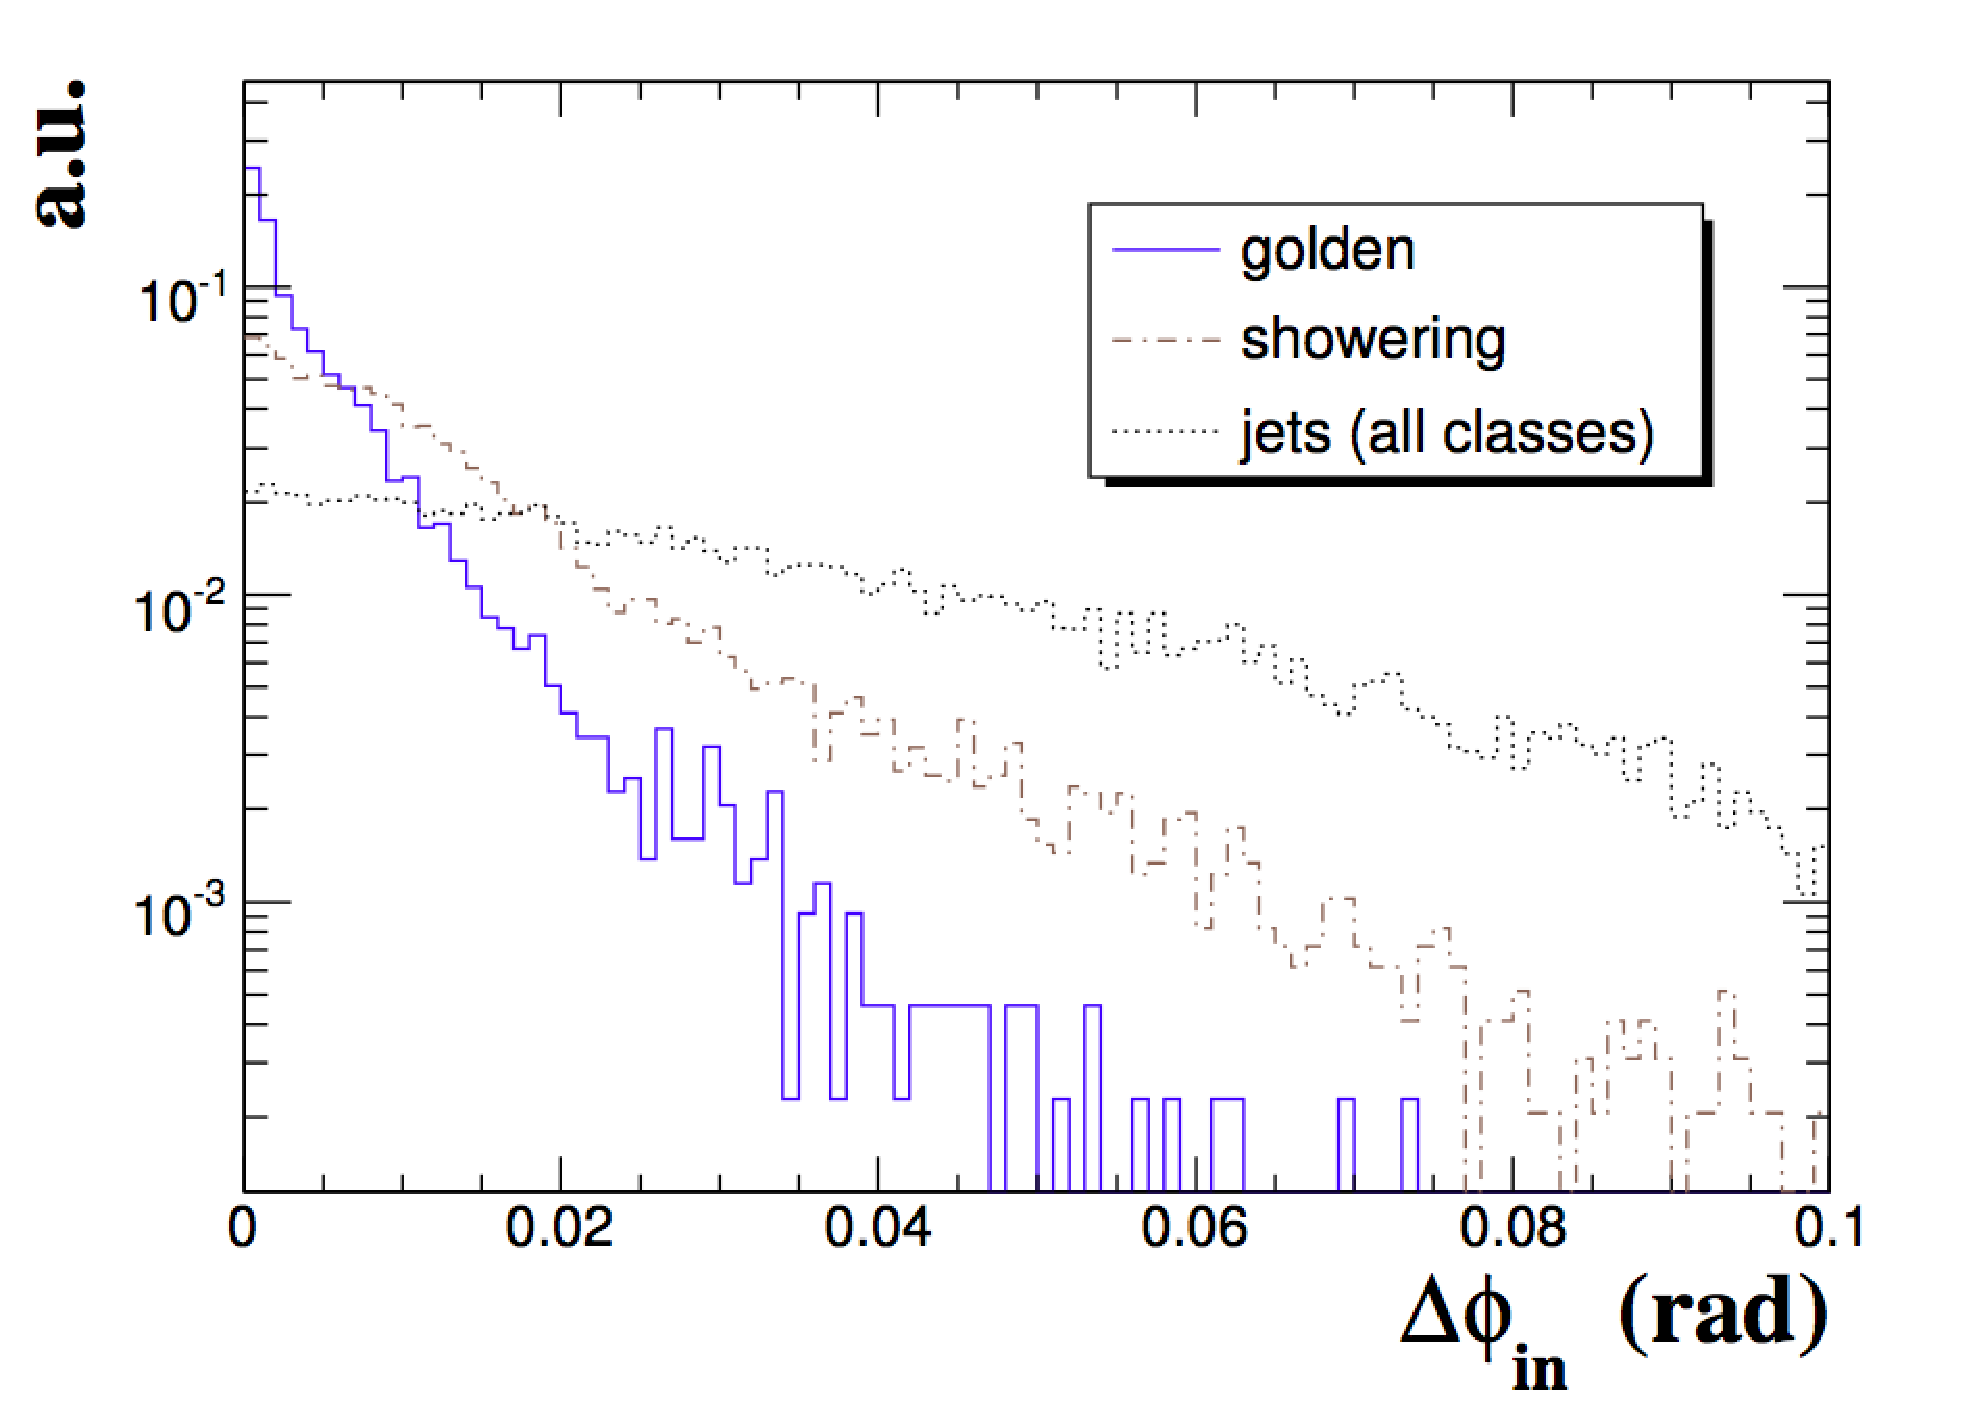
\includegraphics[width=0.5\textwidth]
      {plots/reco/elec-dphi.pdf}}
\subfloat[]{
    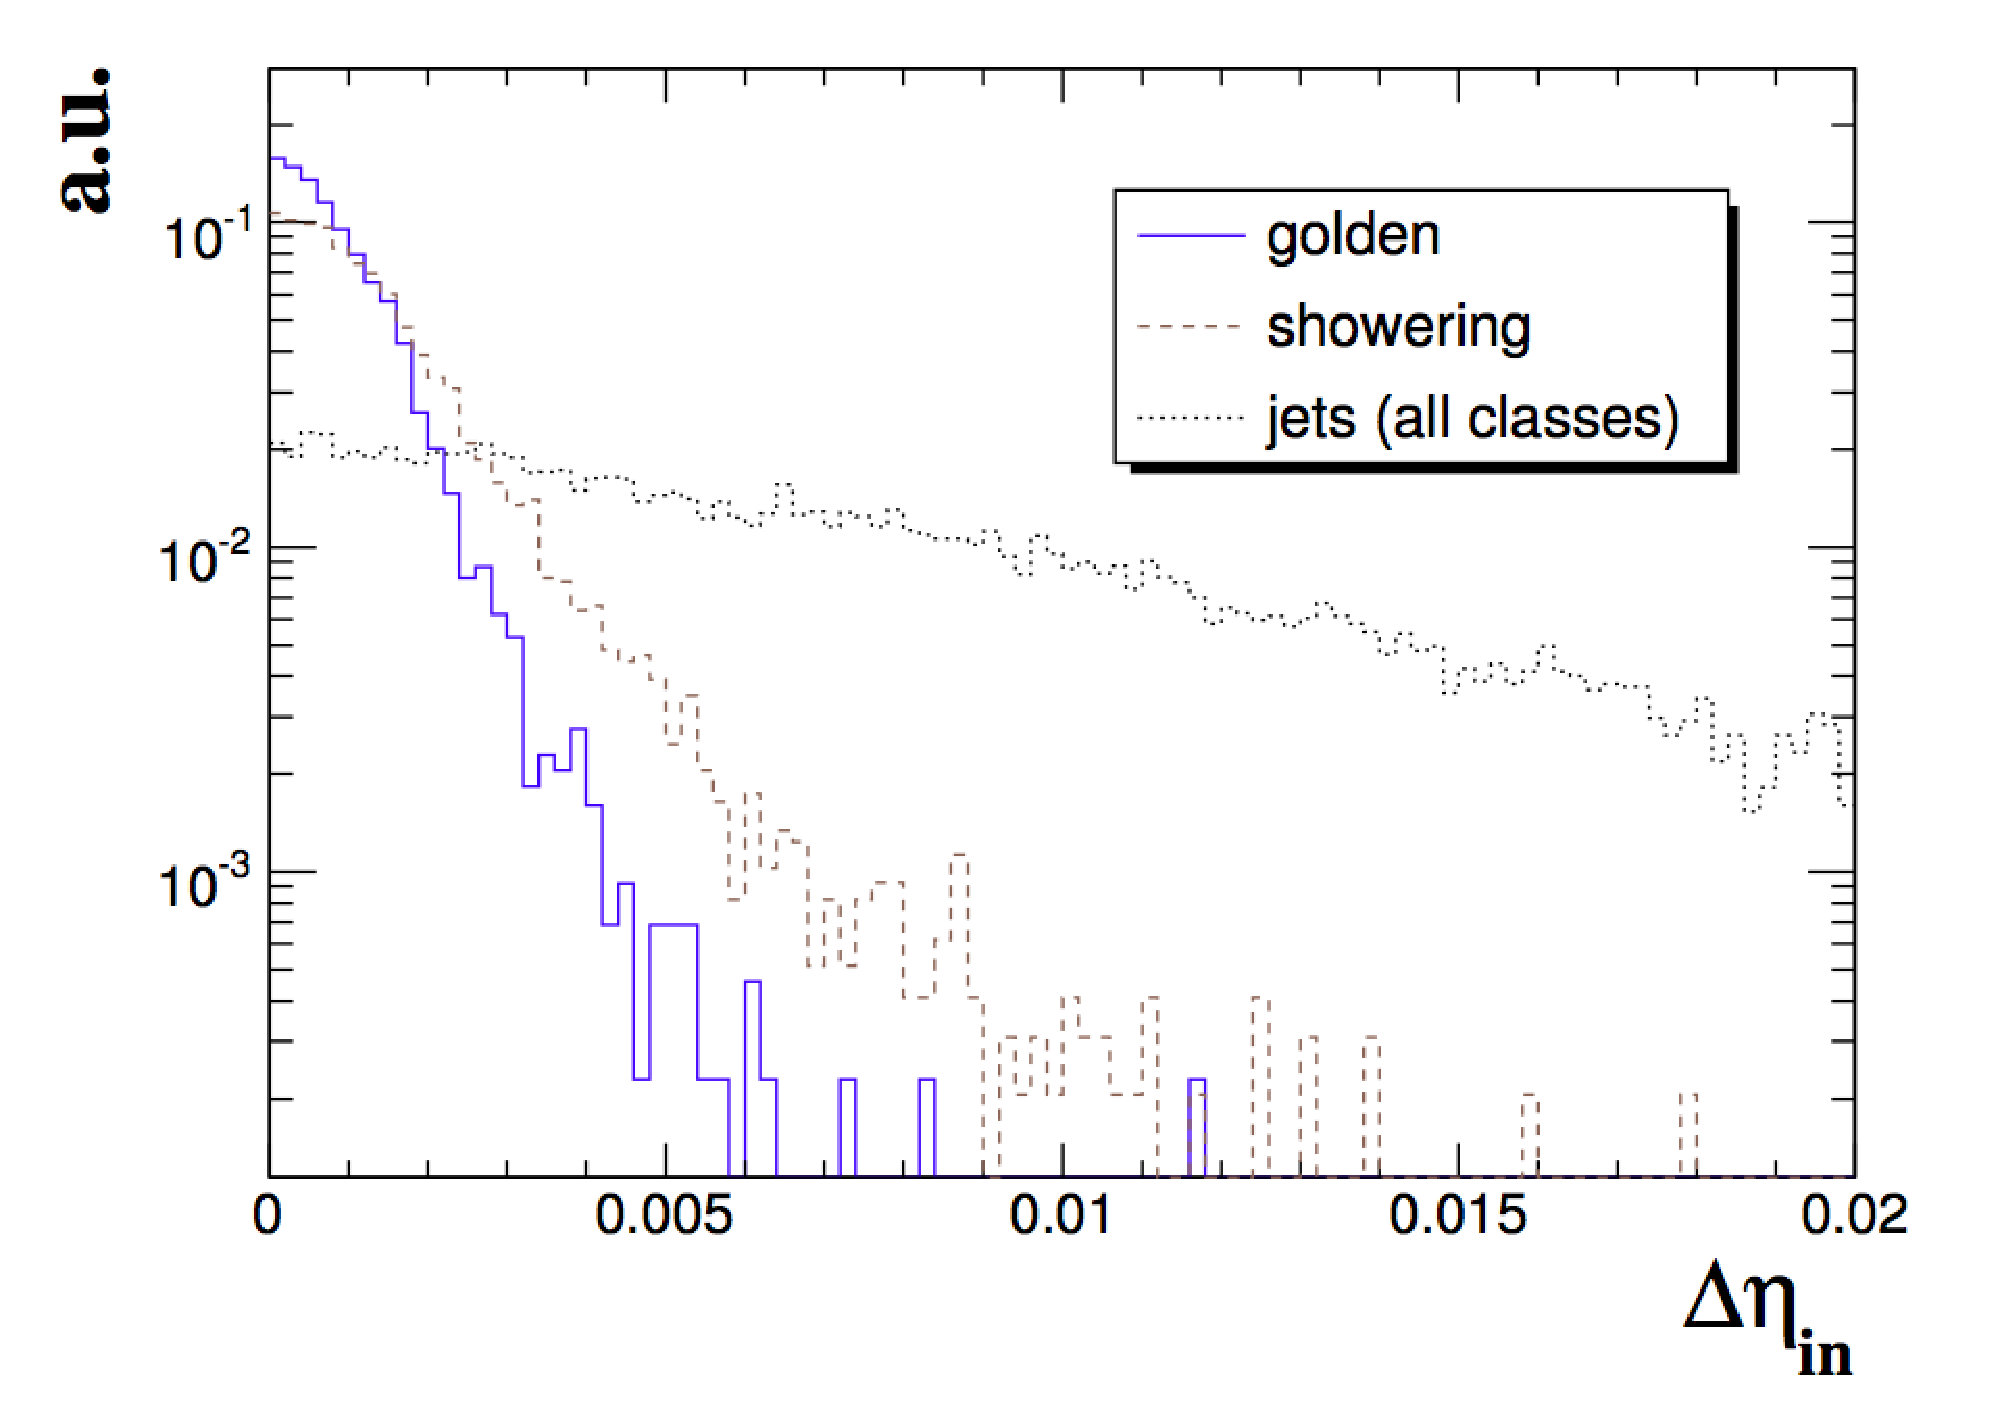
\includegraphics[width=0.5\textwidth] 
      {plots/reco/elec-deta.pdf}} 

\subfloat[]{
    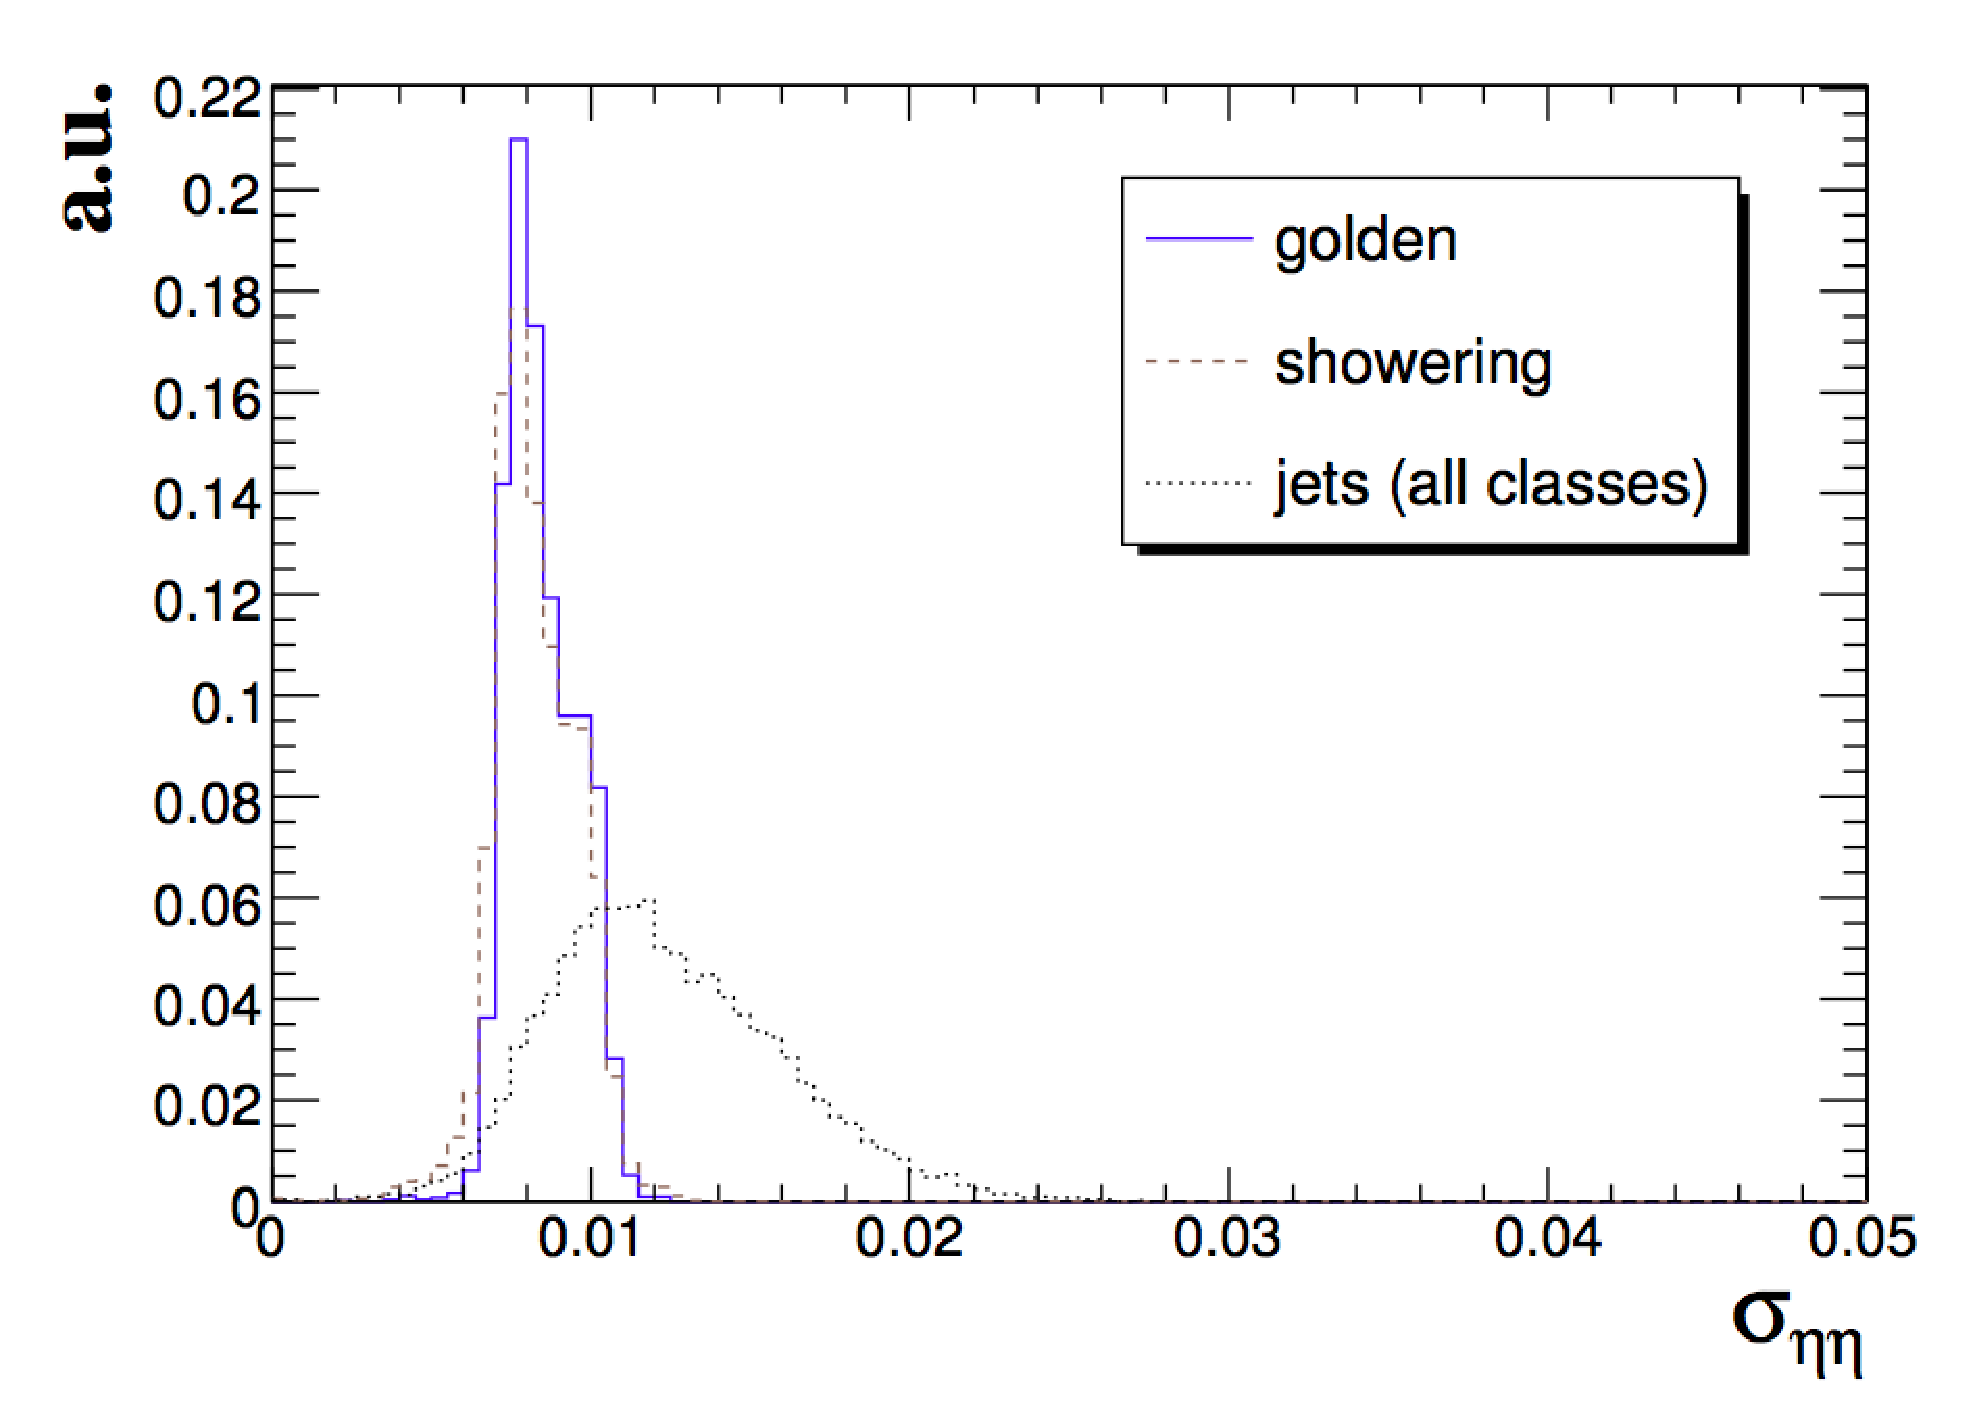
\includegraphics[width=0.5\textwidth]
      {plots/reco/elec-sigieie.pdf}}
\subfloat[]{
    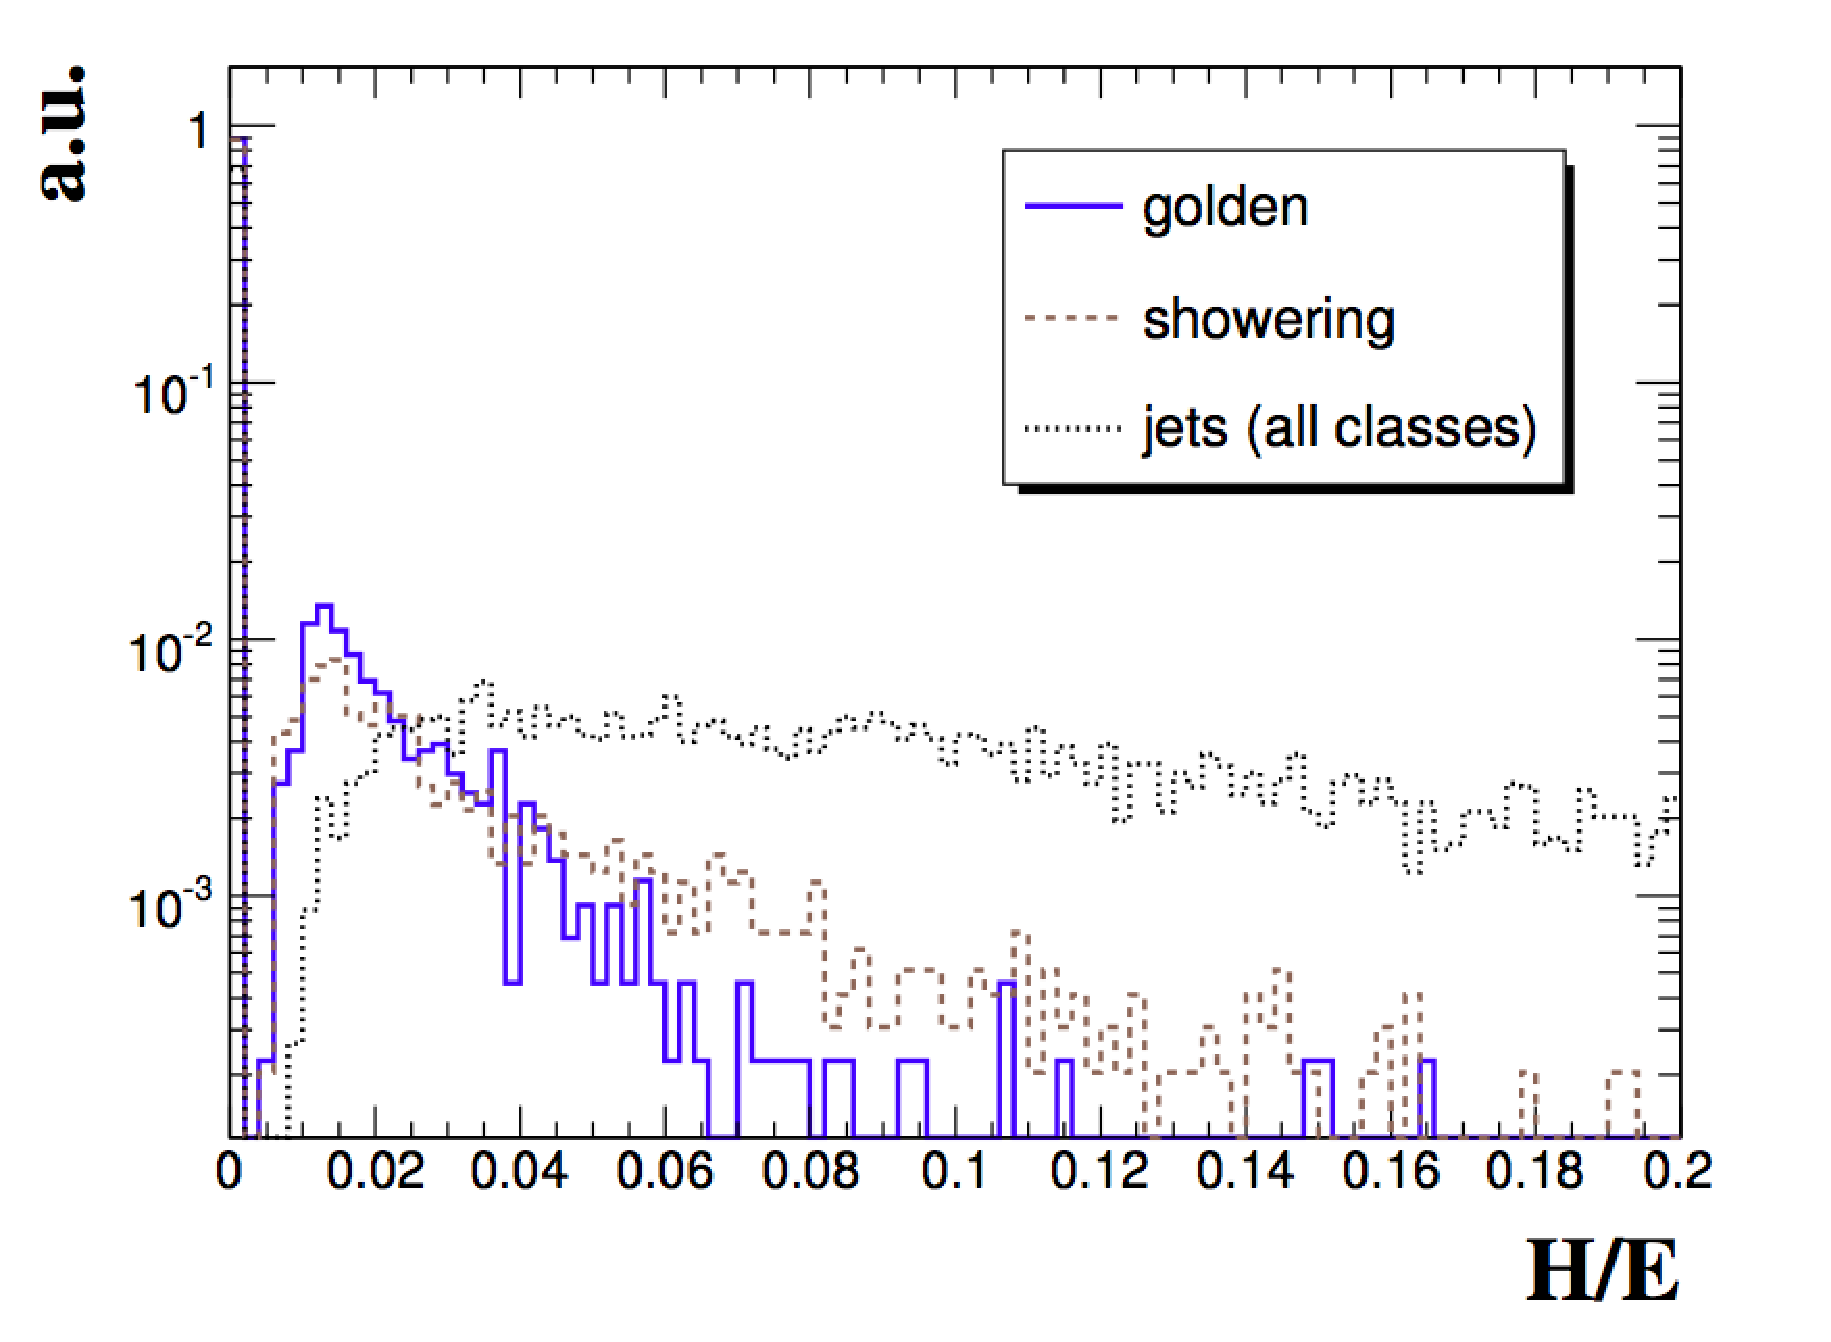
\includegraphics[width=0.5\textwidth]
      {plots/reco/elec-HE.pdf}} 
\end{center}
\caption{
    Plots showing: the separation in a) $\phi$ and b) $\eta$ between the supercluster and the
    track direction, c) the energy-weighted $\eta$ width of the cluster and d)
    the ratio of hadronic and electromagnetic energy in the region of the seed
    cluster. Plots are shown for electrons and backgrounds from jets. 
}
\label{fig:electronID}
\end{figure} 

Conditions on the track quality and kinematic variables can also improve the
efficiency of electron identification. The exact criteria used in the $\PH \to
\Pgt\Pgt$ analysis are described in section \ref{chap:httSM}.

\section{Muons}
\label{sec:muons}

Muons typically travel through the CMS calorimeters with minimal energy deposit
and are reconstructed in the muon chambers. Thus we are able to reconstruct
muons in two independent places - the tracker and the muon chambers. This
greatly improves the ability to isolate muons from hadronic activity. The
``global'' muon reconstruction algorithm \cite{MuonReco} uses both sets of information by
starting from each track in the muon chambers and searching for a compatible
track in the inner tracker. If a compatible track is found, the energy and
momentum of the muon is determined by a fit to the hits in both the inner
tracker and the muon chambers, taking into account the expected energy loss
within the magnet. This improves the momentum resolution compared to
the track only measurement for muons with $\pt$ larger than 200 $\GeV$. For
lower $\pt$ muons, the momentum resolution is driven by the fit to the tracker
hits. For low $\pt$ muons ($< 5~\GeV$), the reconstruction starting from the inner
tracker is more efficient due to the lower probability of these muons reaching
the muon chambers. This is known as ``tracker'' muon reconstruction.  

Backgrounds to prompt muons consist of non-prompt muons from in-flight decays of
hadrons and punch-through of charged hadrons which pass through the calorimeters
into the muon chambers. These backgrounds are reduced through the use of ID
requirements based on the properties of the muon track. In flight decays are
reduced by the requirement of hits in at least one pixel detector and $5$
tracking layers. The $\chi^{2}$ of the global track fit must be better than
$10$, and the global track fit must include hits from at least one segment in
the muon detector, both of which provide rejection of punch-through hadrons. In
addition, track segments must be found in at least two stations of the muon
detector. These conditions taken together provided the ``tight'' muon ID used in
many analyses. The efficiency of CMS muon reconstruction is found to be better
than $96\%$ for muons with $\pt > 10~\GeV$. Some studies of the ID efficiency of
muons in data and \ac{MC} in the context of the $\PH \to \Pgt\Pgt$ analysis can
be found in section \ref{sec:datamcfactors}.

\section{Jets}
\label{sec:jets}

Jets result from the large numbers of quarks and gluons present in a hadron
collider. The term `jet' is used to refer to the collimated shower of particles
which is produced from the hadronisation of such a quark or gluon. In order to
reconstruct the original parton, these showers of particles need to be collected
and combined correctly. Before describing how this is done we must discuss an
important algorithm which allows us to do this successfully. 

\subsection{Particle Flow}
\label{sec:particleflow}

CMS uses a \ac{PF} \cite{CMS-PAS-PFT-09-001,CMS-PAS-PFT-10-001,CMS-PAS-PFT-10-002} 
algorithm to combine the individual track and energy deposits in each sub-detector. 
This allows the reconstruction of individual particles emerging from all vertices: charged
hadrons, neutral hadrons, photons and the muons and electrons already discussed.
These particles can then be 
used to calculate the missing transverse energy $\MET$,
reconstruct jets and quantify the isolation of leptons and photons. A separate
algorithm is used to reconstruct hadronic decays of taus, discussed in section
\ref{sec:taus}. 

The success of the \ac{PF} algorithm is to combine the high resolution of
the tracker with the energy resolution and high granularity of the calorimeters.
The output of the algorithm is a set of the stable particles in the event
resulting from the hard interaction, from the inputs of charged particle tracks,
calorimeter energy deposits and muon chamber hits. The clustering of energy
deposits is performed separately in the \ac{ECAL} and \ac{HCAL}, for electrons
as discussed in section \ref{sec:electrons} this allows the combination of
bremsstrahlung photons with the parent electrons and in the \ac{HCAL} this
allows the separation of the neutral and charged hadrons. The clustering
proceeds by first defining a cluster seed, which corresponds to the calorimeter
cell with the highest local energy. The threshold for clustering neighbouring
cells is that they must have energy greater than 2 standard deviations above
noise level. After the clustering the different \ac{PF} elements are linked into
blocks to be interpreted as a particular particle. This can be done using
extrapolation of tracks into the calorimeters, where the two elements are linked
if the track falls inside the cluster volume.

\subsection{Jet Identification by Clustering}
\label{sec:jetID}

Jets are composed of a wide range of particle types which interact in the
detector in different ways. These particles must be combined using a clustering
algorithm. The choice of algorithm defines how the particles should be combined
taking into account the distance between the objects. In particular the
algorithm should be infrared- and collinear- safe, meaning that the jet
reconstruction is not affected by soft \ac{QCD} radiation or gluon splitting.
The algorithm used for the
analyses in this thesis is the `anti-$k_{\text{T}}$' algorithm as implemented in
the \textsc{fastjet} package \cite{Cacciari:fastjet1}, which considers all 
objects within a certain jet `size' defined by a parameter $R=0.5$, and 
sequentially combines them starting from the one with the
smallest distance from the beamline. If this distance is smaller than the
distance between this object and the closest second object then the first is
taken to be a final state jet and removed from the object list,
otherwise the two objects are combined into one and the process repeats. 
This process is repeated for all objects until none remain in the list. The effect of this
is to form a cluster around the hardest particles in a cone in $\eta$-$\phi$.

Jet identification criteria are applied to reduce the contribution of jets from
noise in the calorimeters. These include the following:
\begin{itemize}
\item Jets must consist of at least one \ac{PF} component. 
\item It is required that the jet energy has contributions
from both the \ac{ECAL} and \ac{HCAL}.
\item The fraction of the total jet energy as a result of photons or neutral
hadrons should be less than 0.99 of the total jet energy.
\item Jets within the acceptance of the inner tracker must have at least one
charged object and a charged energy fraction greater than zero and an electron
energy fraction less than 0.99. 
\end{itemize}

\subsection{Jet Energy Corrections}
\label{sec:JEC}

An important aspect of jet identification is the correct measurement of the jet
energy, which is typically different between reconstructed and true hadron-level jet energy
due to experimental effects. This can be due to uninstrumented regions of the
detector, non-linear calormeter responses and contamination by jets from \ac{PU}
interactions. Particles from different pileup vertices can be clustered and identified as a
jet, or overlap with a jet from the primary vertex affecting the measurement of the jet energy.
Pileup jet identification (ID) is used to classify these events, which consists
of a \ac{BDT} \cite{TMVA} with input variables such as
momentum and spatial distribution of the jet particles. In addition
a calibration factor is applied to account for imperfections in the
neutral-hadron calibration, the jet energy containment and small differences
between the simulated and observed response.

A correction to the jet energy scale is derived
\cite{CMS-JME-10-011}:

%Read this paper when you have internet and find a better way to write this
%equation

\begin{equation}
P_{\text{corr}}^{\mu} = C_{\text{PU}}(\pT^{\text{raw}},\eta) \cdot
C_{\text{rel}}(\pT^{\text{PU}},\eta) \cdot C_{\text{abs}}(\pT^{\text{rel}},\eta) \cdot
P_{\text{raw}}^{\mu}\, .
\end{equation}

In this equation, $C_{\text{PU}}$ is the correction for \ac{PU},
$C_{\text{rel}}$ is a relative correction and $C_{\text{abs}}$ is an absolute
correction. The corrections are applied sequentially such that the \ac{PU}
correction is a function of raw jet $\pt$, the relative correction is a function
of the $\pt$ corrected for the pileup effects ($\pt^{\text{PU}}$) and finally
the absolute correction is a function of the relative-corrected $\pt$
($\pt^{\text{rel}}$). All of the corrections are also applied as a function of
jet $\eta$. These subsequent corrections are applied to the raw
4-vector of the jet $P_{\text{raw}}^{\mu}$ to yield the corrected 4-vector
$P_{\text{corr}}^{\mu}$.

The \ac{PU} correction is determined using the $\pt$ density in the event to
estimate the contribution from \ac{PU} on a per-jet basis. The relative
correction is determined using a dijet $\pt$ balance method which uses dijet
events containing a jet with $|\eta| < 1.3$ and exploits momentum conservation.
The probe jet (which can have any value of $\eta$), is used to calculate the
average of a balance quantity, defined as:
$(\pT^{\text{probe jet}}-\pT^{\text{ref jet}})/\pT^{\text{average}}$, in bins of
average dijet $\pt$ and probe $\eta$. Figure \ref{fig:jetresponse} shows the
values of the response for \ac{MC} and data. The absolute correction is measured
using the \ac{MPF} method \cite{Abe:1992sj}, using $\gamma$+jets and $\PZ$+jets
events and enforcing momentum conservation in light of the fact that these
events shouldn't contain any real $\MET$. Thus any measured $\MET$ can be used to
calibrate the $\pt$ of the jets. The total uncertainty on the jet energy scale
is given by the sum in quadrature of the estimated uncertainties in each of the
correction factors. This uncertainty varies between approximately $3$ and $5\%$
depending on $\pt$ and $\eta$. 

%could add a JES uncert plot here.

\subsection{B-tagged jets}
\label{sec:btag}

The identification of jets which originate from b-quarks is important in many
\ac{SM} and \ac{BSM} processes. As a result of the fact that decays of b-quarks
are suppressed by small CKM matrix elements, b-flavoured hadrons have relatively
long lifetimes. These hadrons are also relatively heavy due to the large mass of
the b-quark, and as such the decay products typically have large momenta
perpendicular to the b-hadron momentum direction. Both of these features are
exploited in identification of b-tagged jets.

In the $\PH \to \Pgt\Pgt$ analysis, jets originating from b-quark
hadronization are identified using the combined secondary-vertex b-tagging
algorithm \cite{bjets}. The long lifetime of the b-hadrons results in a
secondary decay vertex which can be reconstructed.
%some more to be added about CSV and b-tag uncertainties. 

\section{$\MET$}
\label{sec:met}

Neutrinos and any other hypothetical weakly interacting stable particles do not
interact with the CMS deterctor. We infer their production from the resulting
imbalance in $\ET$ in a given event, which the hermeticity of the CMS detector
allows us to measure to a high degree of accuracy. This is crucial not only in
many searches for new physics involving such hypothetical particles, but also for
\ac{SM} processes involving neutrinos. In particular for the $\PH \to \Pgt\Pgt$
analysis accurate measurement of the $\MET$ is essential to reconstruct the
candidate taus after they decay via the weak interaction.

The \ac{PF} algorithm allows us to calculate $\MET$ as the opposite of the vectorial sum
of the transverse momenta of all \ac{PF} particles. The resolution of this PF
$\MET$ degrades rapidly with pileup. A more precise
measurement of $\MET$ can be achieved with so-called `MVA
$\MET$', which uses a \ac{BDT} regression multivariate analysis
including the \ac{PF} $\MET$ as one input. Other inputs are versions of the
$\MET$ calculated using the following combinations of \ac{PF} particles: 
\begin{itemize}
\item charged hadrons from the primary vertex;
\item charged hadrons from the primary vertex and neutral particles in jets
passing the pileup jet ID;
\item charged hadrons from pileup vertices and neutral particles in jets failing
the pileup jet ID;
\item charged hadrons from the primary vertex and all neutral particles in the
event, to which is added the vectorial sum of the transverse momenta of neutral
particles within jets failing the pileup jet identification.
\end{itemize}

The MVA $\MET$ has a resolution which is much less
dependent on pileup, as can be seen in figures \ref{fig:mvamet}.

\begin{figure}
\begin{center}
\subfloat[]{
    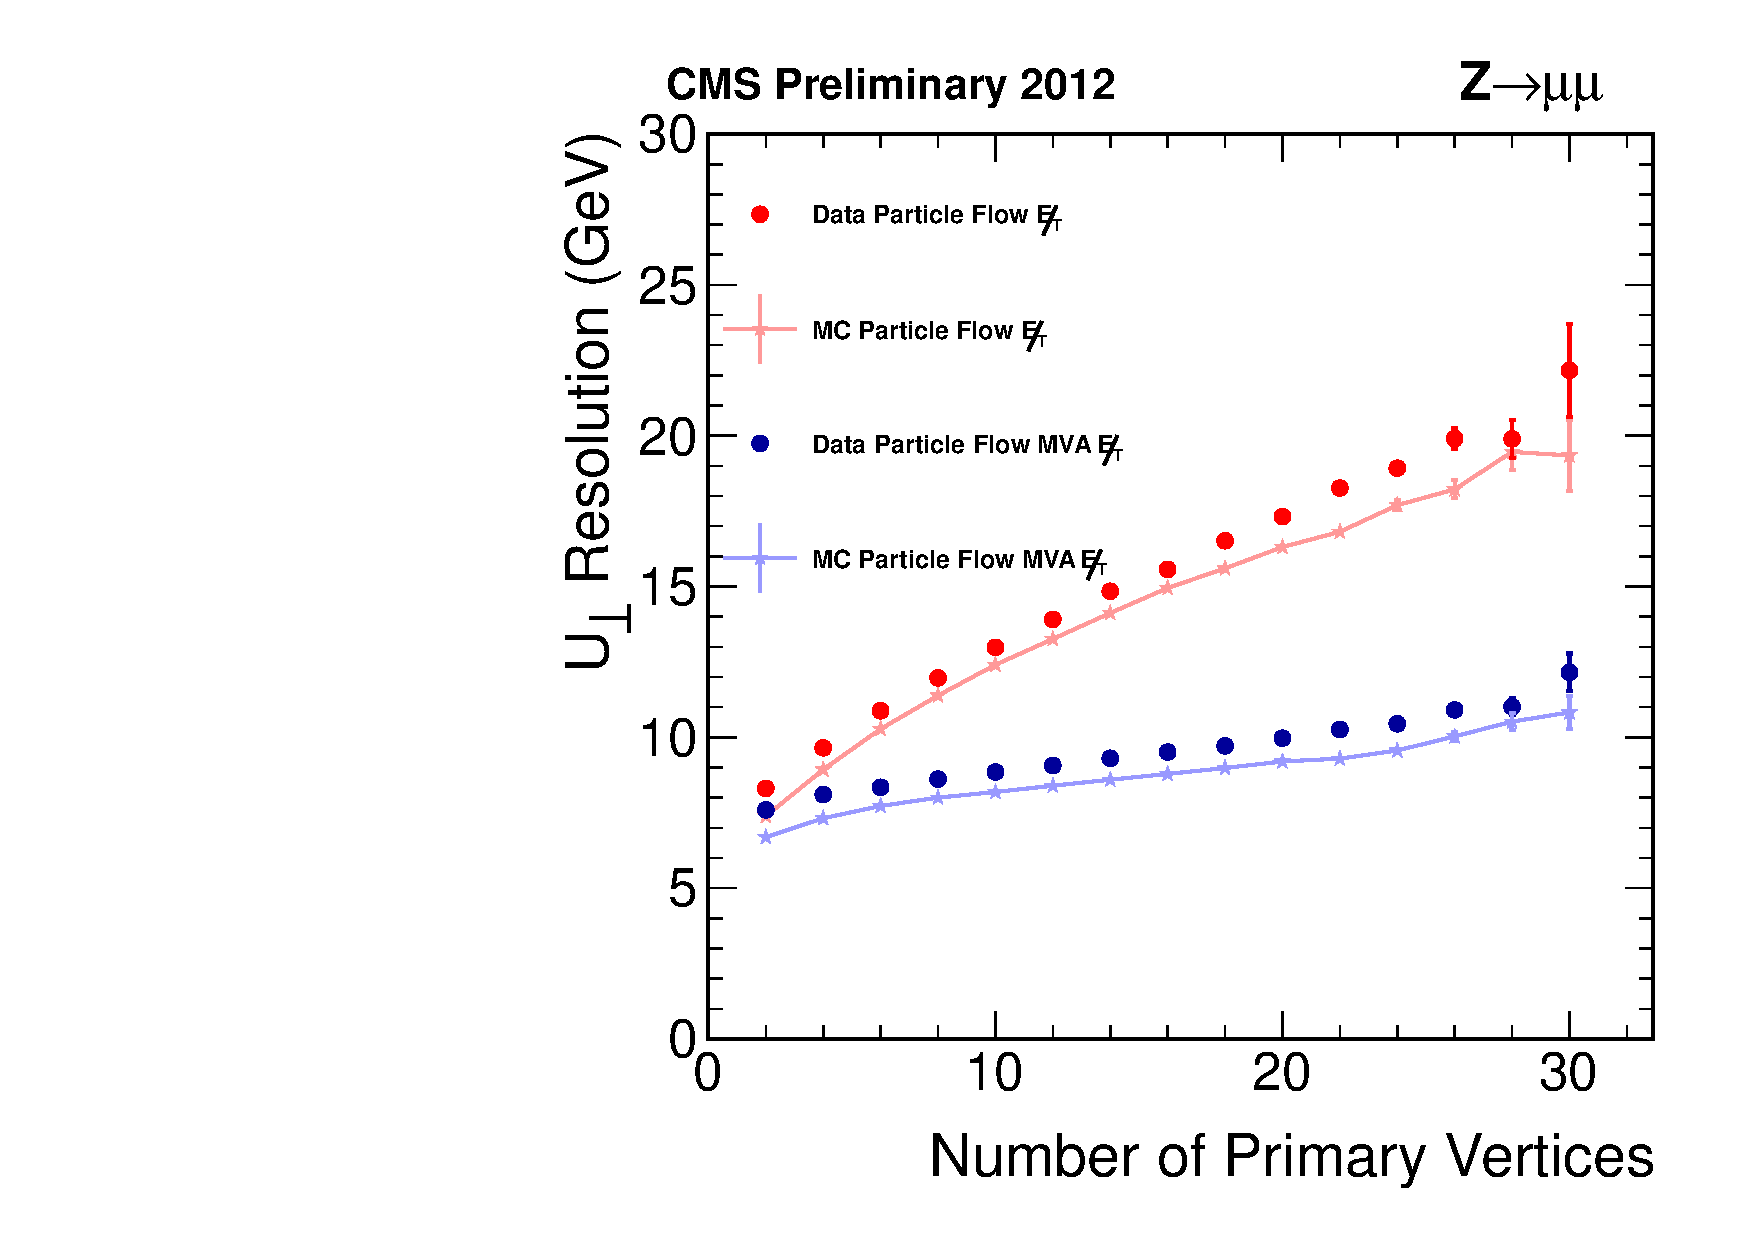
\includegraphics[width=0.5\textwidth]
      {plots/reco/U1Res.pdf}}
\subfloat[]{
    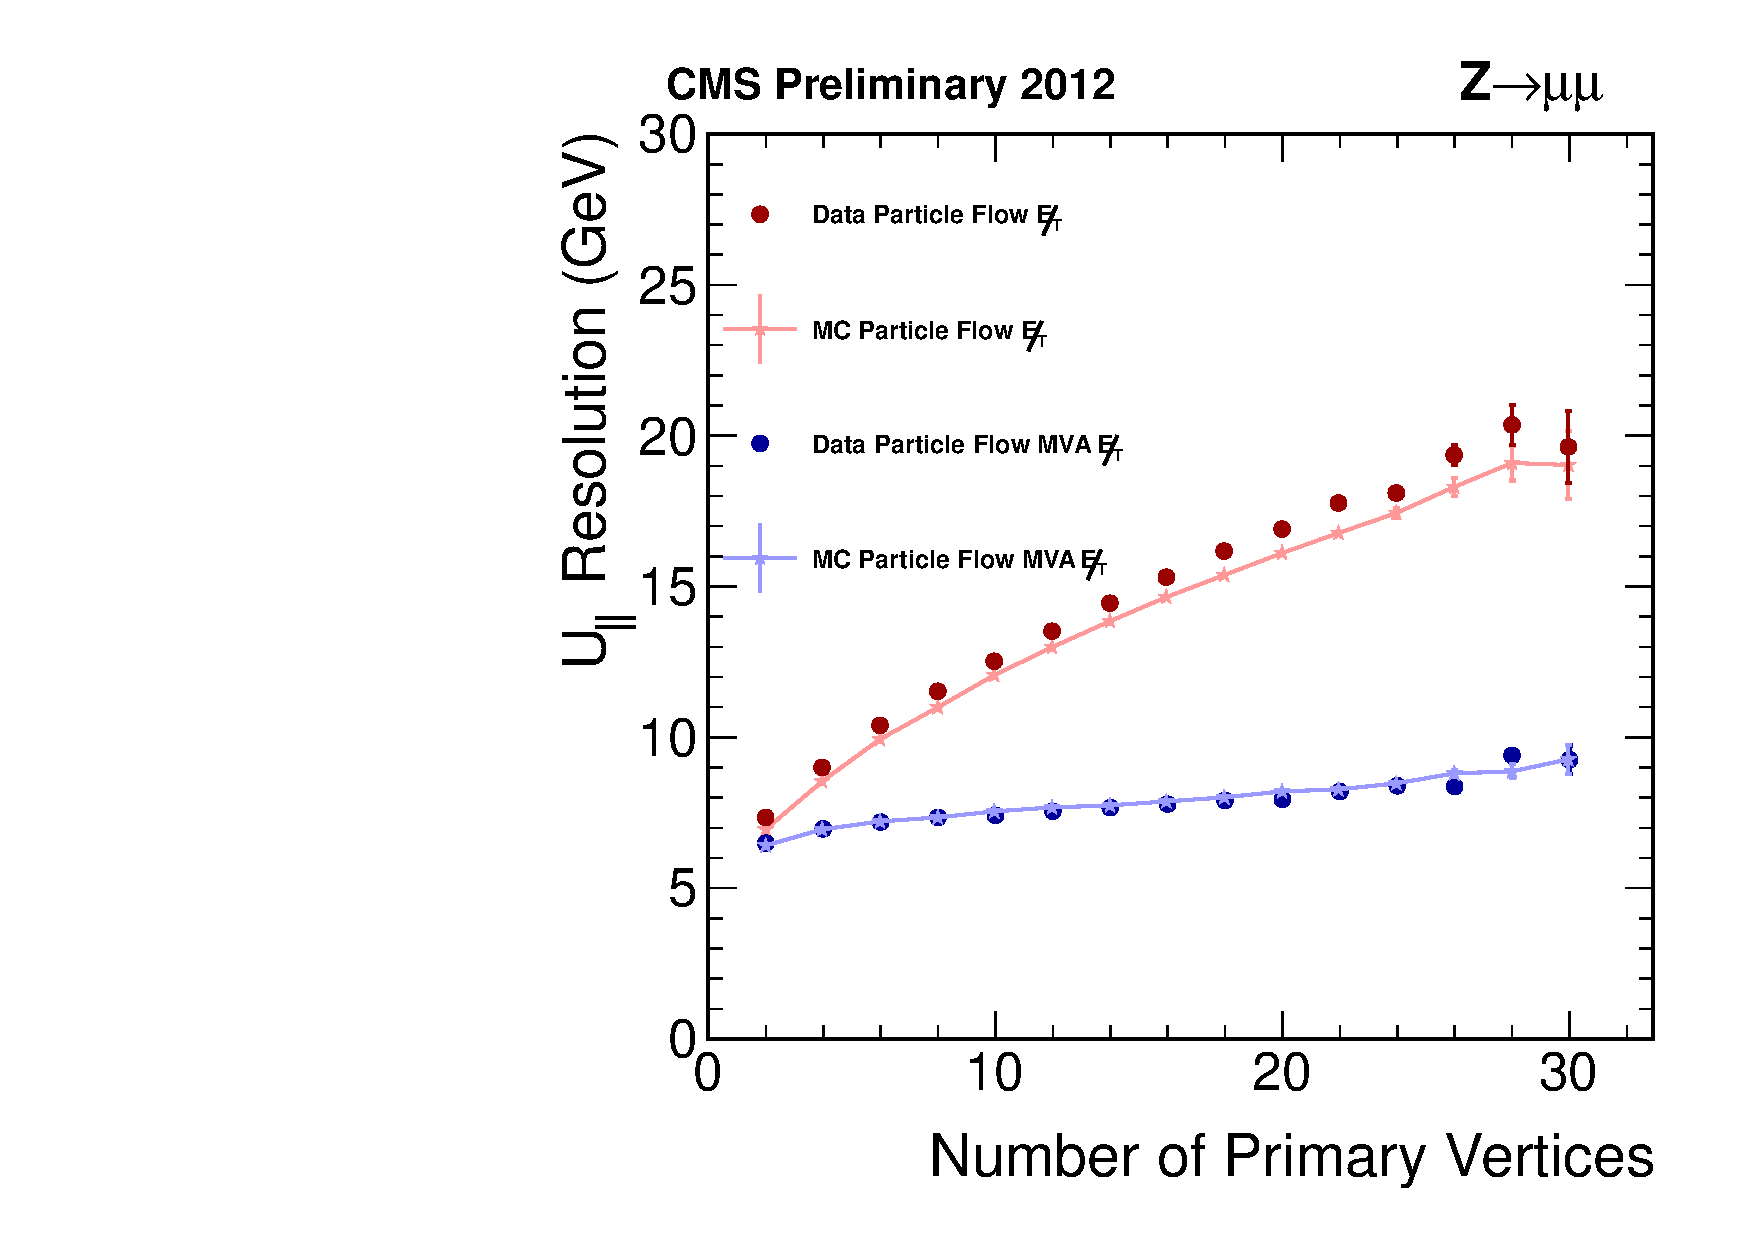
\includegraphics[width=0.5\textwidth] 
      {plots/reco/U2Res.pdf}} 
\end{center}
\caption{Plots illustrating the dependence of $\MET$ resolution on the number of
primary vertices in the event.
}
\label{fig:mvamet}
\end{figure}

\section{Hadronic Taus}
\label{sec:taus}

\section{Di-tau Mass Reconstruction in $\PH \to \Pgt\Pgt$}
\label{sec:svfit}

Reconstruction of the full di-tau mass gives us the mass of the Higgs candidate.
This reconstruction is made less straightforward by the fact that the taus
themselves decay. We can simply combine the visible products to evaluate a quantity known as
visible mass, but greater accuracy is achieved if the full mass can be
reconstructed including the invisible neutrinos. This can be achievied
using a likelihood based algorithm called SVFit, which combines the visible decay products 
and the reconstructed $\MET$.

Figure \ref{fig:svfit} shows the separation between signal and $\PZ \to \Pgt\Pgt$
background in the case of using the visible mass or the mass from SVFit. It can
clearly be seen that the shape separation is greatly improved in the SVFit case.
The improvement in expected limit from using SVFit over visible mass in the $\PH
\to \Pgt\Pgt$ analysis is around 40$\%$.


\begin{figure}
\begin{center}
\subfloat[]{
    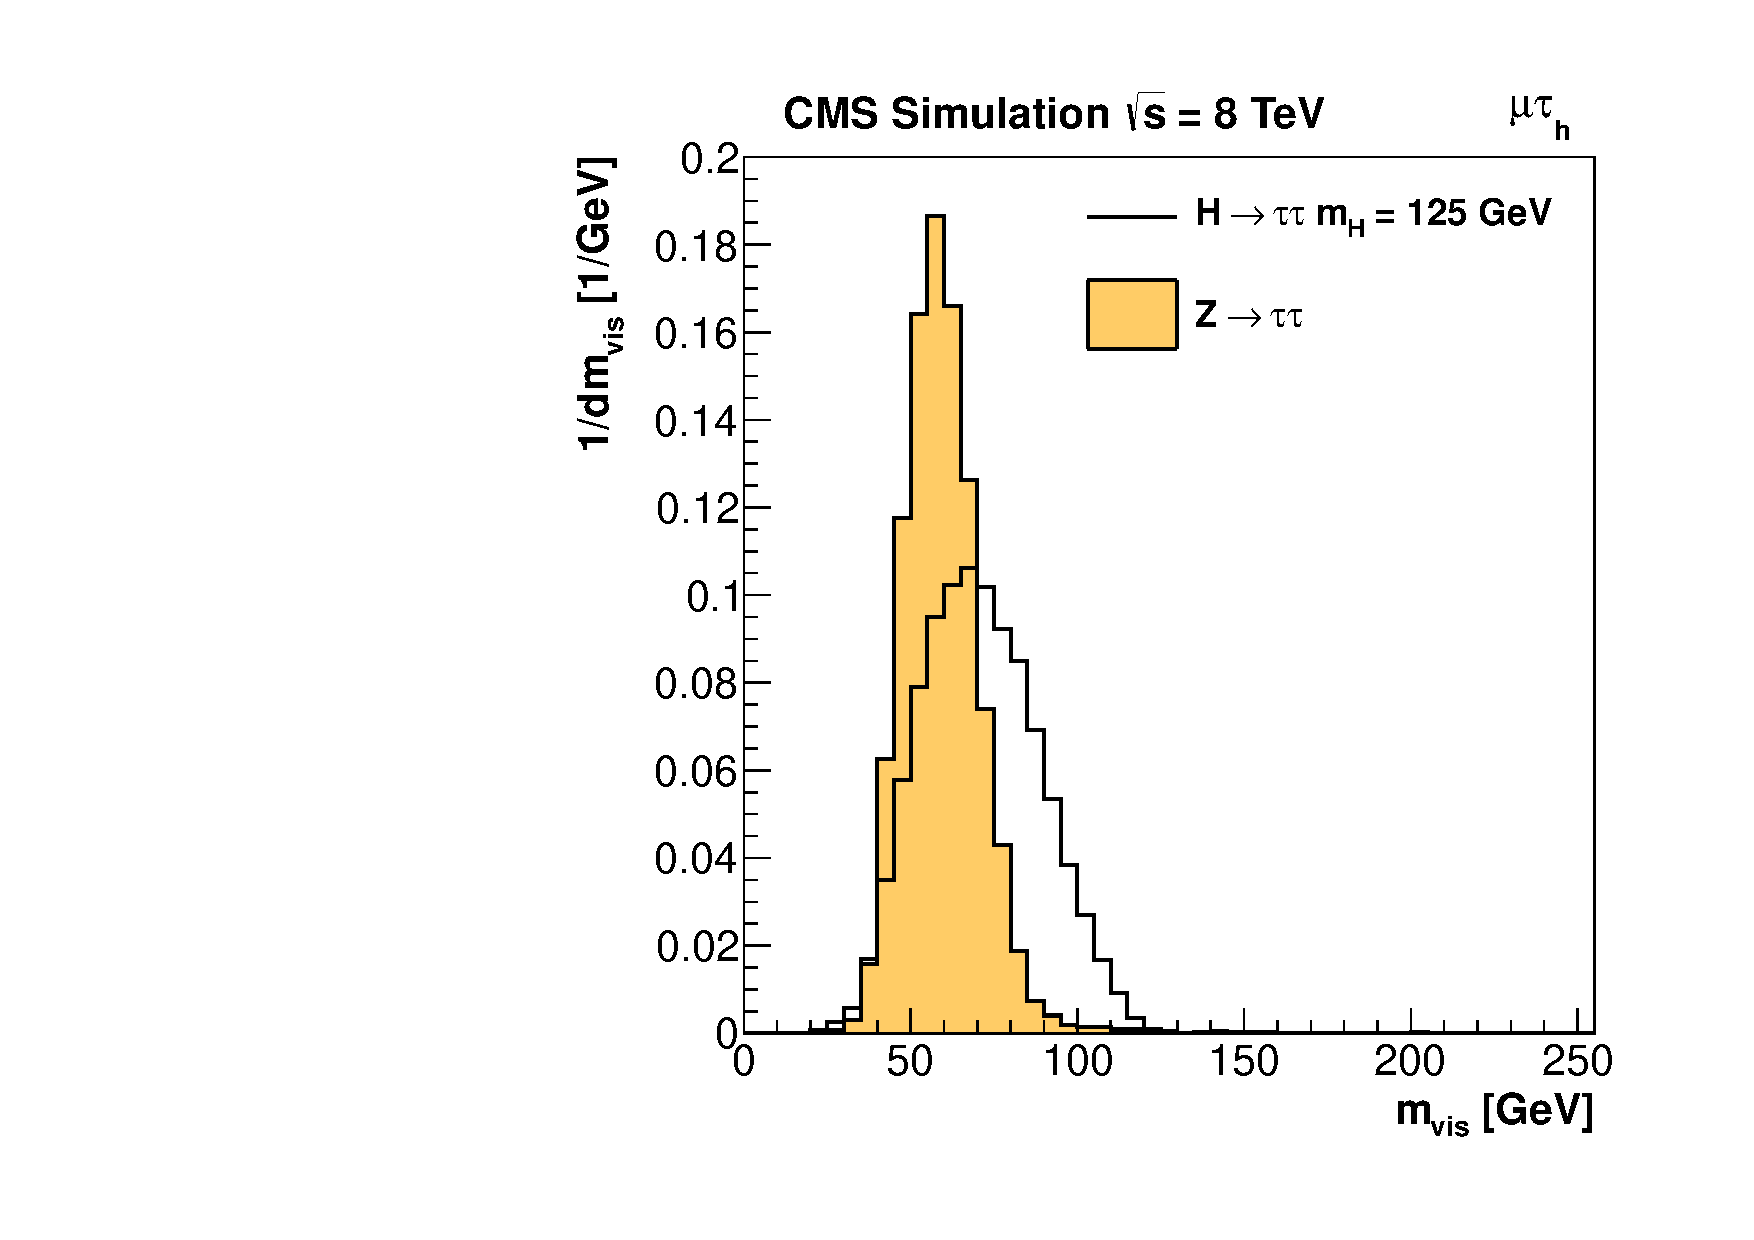
\includegraphics[width=0.5\textwidth]
      {plots/reco/svFitPerformance_forColin_visMass.pdf}}
\subfloat[]{
    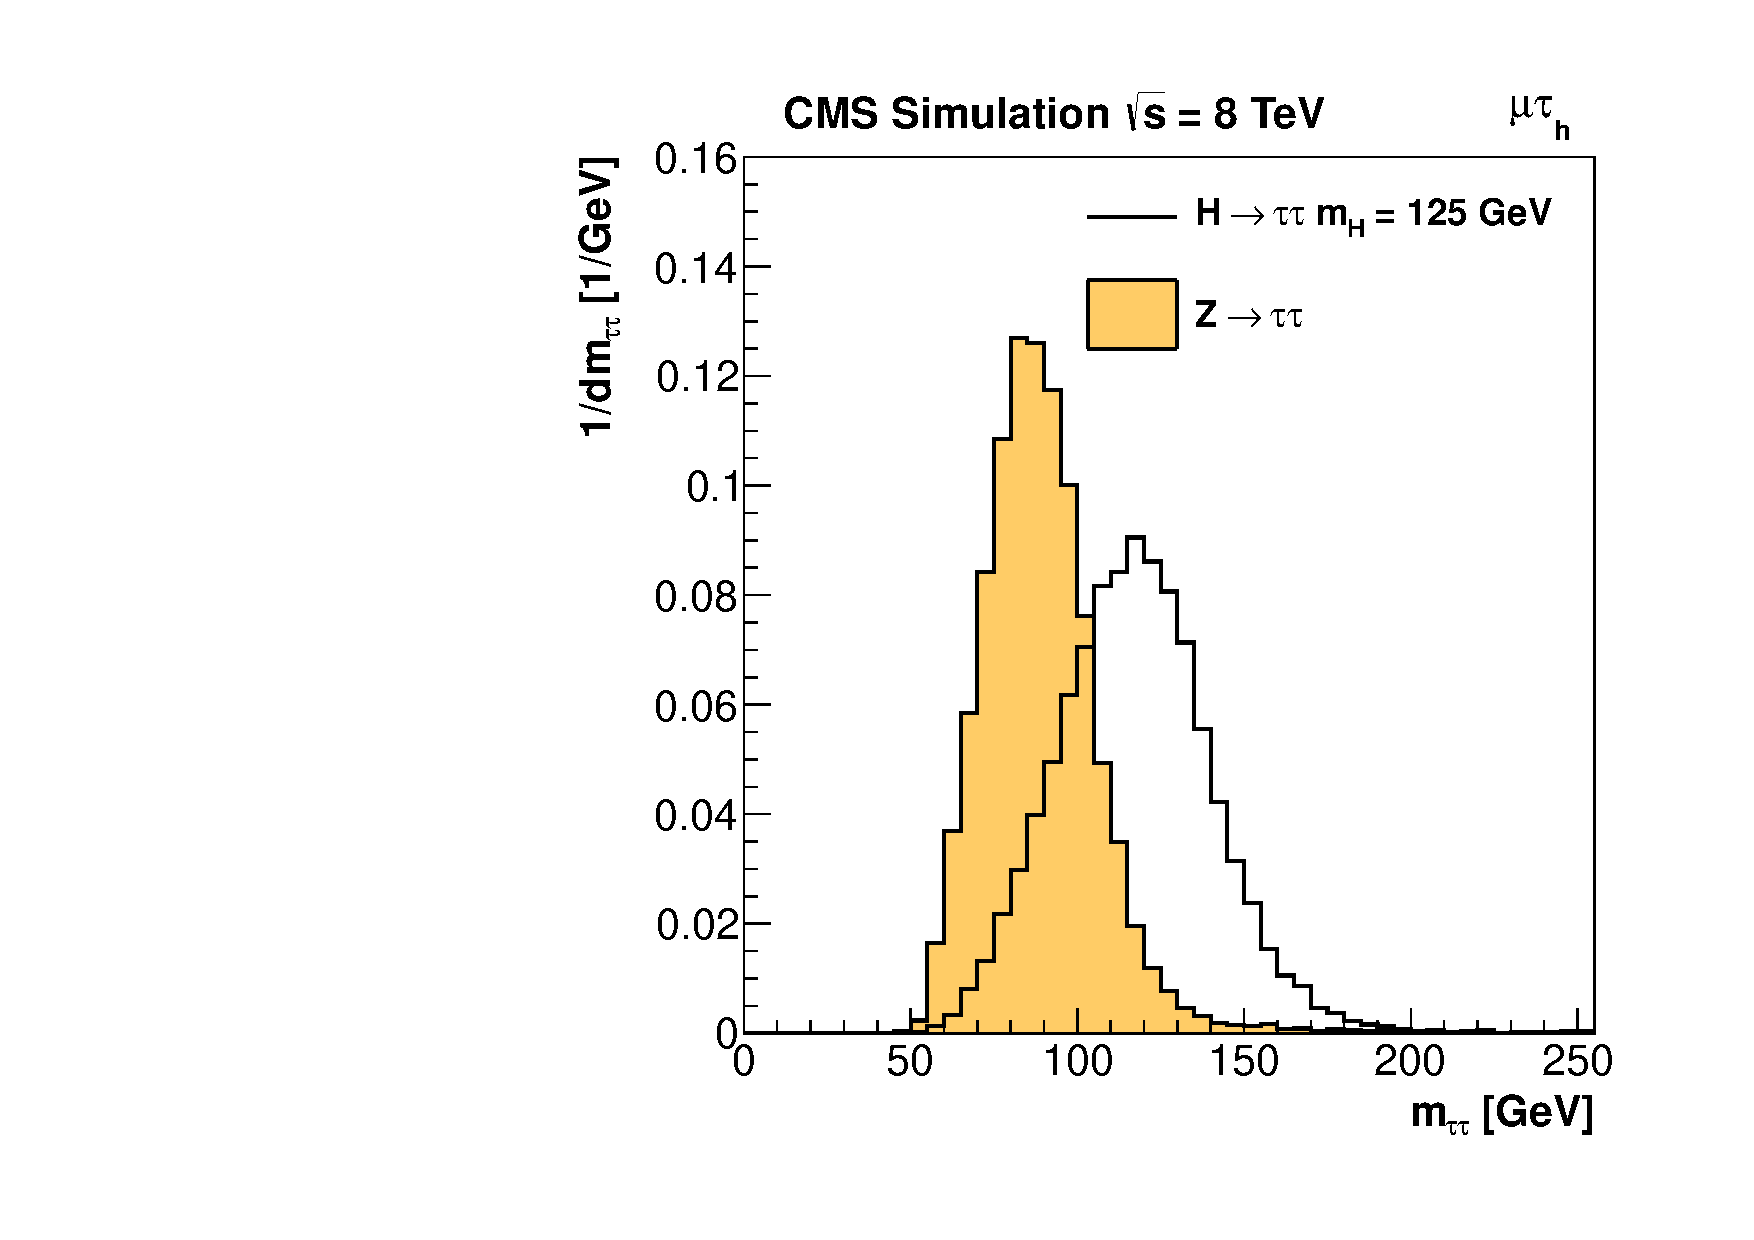
\includegraphics[width=0.5\textwidth] 
      {plots/reco/svFitPerformance_forColin_svFitMass.pdf}} 
\end{center}
\caption{
}
\label{fig:svfit}
\end{figure}

\section{\ac{MC} simulation of signal and backgrounds}

To model the contributions of signal and background events in the analysis
Monte-Carlo (MC) simulation is used. Simulation of signal events is generated
using POWHEG \cite{powheg} interfaced to PYTHIA \cite{pythia}, and of
background events using MADGRAPH \cite{madgraph}. Pileup is simulated using
additional interactions from PYTHIA and reweighting the simulated events to
match the observed pileup distribution in data, which is different depending on
the run period. In addition, the $E_{\rm{T}}^{\rm{miss}}$ response in
simulation is corrected for the $E_{\rm{T}}^{\rm{miss}}$ energy scale and
resolution which is measured in $Z\rightarrow\mu\mu$ events. The generated
events are then processed through a simulation of the CMS detector based on
GEANT4 \cite{geant4} and are reconstructed with the same algorithms used in
data.



